\section{Implementation and Supplementary Results}

\subsection{Wang data preparation}
\label{sec:wang_data}

We reconstruct item means from the public participant-rating exports. For each dimension, we average finite numerical responses in the original 1--7 range, excluding 11 invalid familiarity cells and one invalid metaphoricity cell. Text matching uses Unicode normalization and whitespace removal. We retain items with ratings on all three dimensions and omit four whose texts differ between the material list and the rating headers: families 44 and 93 (familiarity), 98 (metaphoricity), and 104 (meaningfulness). The retained set contains 119 novel metaphors, 119 similes, and 118 literal sentences across 120 families. Our targets are these reconstructed export means; equivalence to the original study's final norms, including its participant exclusion procedure, has not been established.

\subsection{Implementation details}

The rubric-guided LLM uses temperature 0 and returns one continuous score per requested dimension. Each request includes the original expression, a dimension definition, a rating question, and five same-dimension labeled examples retrieved by character TF--IDF cosine similarity. The scorer output is constrained to $[1,5]$ and is parsed as JSON. The evidence prompt returns source and target domains, a mapping relation, and quotations with source positions. Quotations are checked against the original input.

BGE embeddings are 512-dimensional normalized vectors. BGE-KNN uses $k=5$ with neighbor weights $\max(\cos(\mathbf{z}_i,\mathbf{z}_j),0.01)$. BGE-Ridge uses $\alpha=10$. Fusion weights lie on a 0.05 grid, are nonnegative, and sum to one; for each weight vector, the intercept is the median OOF residual clipped to $[-0.5,0.5]$. Candidates are selected by MAE, with ties broken by RMSE and then distance to equal weights. The outer-training predictions used to select fusion weights are generated by four inner folds. After selection, semantic predictors are refitted on the complete outer-training portion.

COGMED contributes 671 final outer-test predictions and 2,684 inner OOF predictions per scorer. Wang contributes 356 and 1,424, respectively. The inner OOF records are used for fitting and are not counted as test observations. Model inference used a single RTX 4090. Prompts, run configurations, item IDs, and training-side prediction records are archived with the project.

\subsection{Implementation of the adapted baselines}
\label{sec:adapter_details}

The COGMED comparison evaluates AutoSCORE-adapted and RULERS-adapted on the same 671 outer-test items as CEMS. Item identifiers, human ratings, and outer folds are matched across methods.

For each item--fold combination, retrieved examples exclude the outer test fold, the item's original fold, its own ID, and its family. For a test item, examples can come from the other four folds. The shared rubric is compiled from task definitions without human labels. AutoSCORE-adapted passes extracted components to its scoring agent. RULERS-adapted uses the judge's continuous \texttt{score} field on $[1,5]$; checklist decisions and confidence are auxiliary outputs and are not converted into the reported score. Outputs are parsed as JSON with a score for every rating dimension.

\subsection{Statistical comparisons}
\label{sec:bootstrap_details}

Paired percentile bootstrap intervals use 2,000 replicates. The COGMED component and mapping analyses resample items; the Wang analyses resample the 120 item families. The COGMED adapted-baseline comparisons resample groups with seed 20261029, pairing predictions by item and outer fold. The COGMED analysis set contains 671 groups of one item each, so item and group resampling use the same sampling units. These comparisons use the adapted methods' direct continuous scores and the saved CEMS predictions. No multiple-comparison correction is applied.

\subsection{Backbone results}

\begin{figure*}[t]
\centering
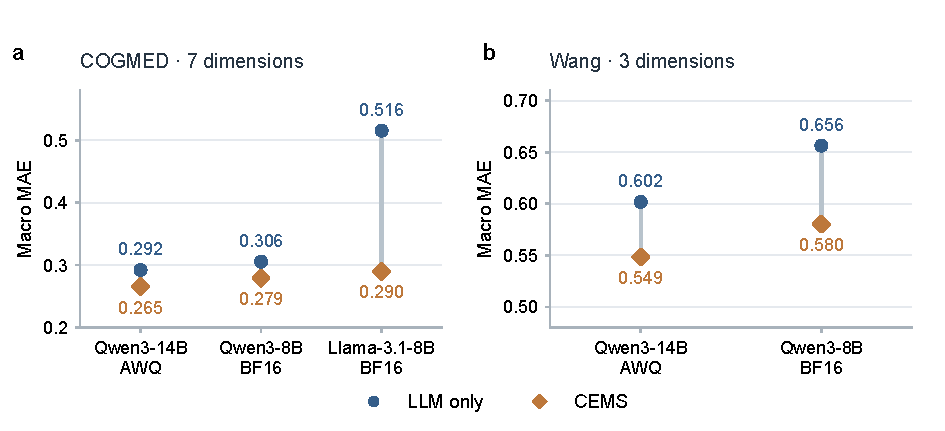
\includegraphics[width=0.88\textwidth]{figures/backbone_comparison.pdf}
\caption{Macro MAE for rubric-guided LLM scores and CEMS across five scorer--task pairs. The two panels use different original rating scales.}
\label{fig:backbones}
\end{figure*}

Table~\ref{tab:backbone_all} reports all five metrics for the five scorer--task pairs. The fusion MAE is lower in every pair. Other metrics vary by task and backbone.

\begin{table*}[t]
\centering
\footnotesize
\setlength{\tabcolsep}{5pt}
\caption{Full macro-averaged results for scorer--task pairs.}
\label{tab:backbone_all}
\begin{tabular}{lllrrrrr}
\toprule
Task & Scorer & Method & MAE & RMSE & Pearson & Spearman & QWK\\
\midrule
COGMED & Qwen3-14B-AWQ & LLM & 0.292 & 0.411 & 0.715 & 0.700 & 0.544\\
COGMED & Qwen3-14B-AWQ & CEMS & 0.265 & 0.361 & 0.750 & 0.721 & 0.537\\
COGMED & Qwen3-8B & LLM & 0.306 & 0.429 & 0.665 & 0.639 & 0.483\\
COGMED & Qwen3-8B & CEMS & 0.279 & 0.381 & 0.713 & 0.681 & 0.484\\
COGMED & Llama-3.1-8B & LLM & 0.516 & 0.721 & 0.493 & 0.516 & 0.374\\
COGMED & Llama-3.1-8B & CEMS & 0.290 & 0.393 & 0.693 & 0.658 & 0.448\\
Wang & Qwen3-14B-AWQ & LLM & 0.602 & 0.810 & 0.829 & 0.750 & 0.793\\
Wang & Qwen3-14B-AWQ & CEMS & 0.549 & 0.745 & 0.827 & 0.736 & 0.796\\
Wang & Qwen3-8B & LLM & 0.656 & 0.867 & 0.813 & 0.745 & 0.745\\
Wang & Qwen3-8B & CEMS & 0.580 & 0.760 & 0.815 & 0.739 & 0.759\\
\bottomrule
\end{tabular}
\end{table*}

\subsection{Wang extension protocol}
\label{sec:appendix_extension}

This exploratory variant replaces BGE-Ridge with a kernel regressor using frozen Qwen3-8B embeddings and applies half-strength isotonic calibration. MAE falls from 0.5485 to 0.5149. The differences from single-LLM isotonic calibration ($-0.0145$, 95\% CI $[-0.0301,0.0012]$) and the supervised-BGE extension ($-0.0109$, $[-0.0248,0.0038]$) have intervals that include zero. The following protocol specifies the representation selection and calibration steps.


The exploratory experiment uses six frozen Qwen3-8B representations: the final-token vector, last-layer mean pooling, and last-four-layer mean pooling, each for the original expression and an expression with a task prefix. Each has 4,096 dimensions. The search includes these six representations and BGE, a linear kernel and RBF kernels with $\gamma\in\{2,8\}$, and regularization values $\{0.001,0.01,0.1,1,10,100\}$, giving $7\times3\times6=126$ settings. We calculate candidate errors on four inner training folds, then refit the selected representation and kernel on the full outer training set.

For each outer fold and dimension, we select the representation, fit fusion weights, and fit isotonic calibration using outer-training labels. Inner predictions from the selected candidate are used to fit the fusion weights. Fusion scores for the outer-training items are then used to fit the monotone calibration map. Outer-test labels are used only for evaluation. The outer test fold stays independent, but the training predictions used for fusion and calibration are not produced by a fully nested cross-fitting procedure.

The supervised-BGE control fine-tunes the encoder with a LayerNorm and three-output linear head. It uses AdamW, learning rates $2\times10^{-5}$ for the encoder and 0.002 for the head, batch size 16, SmoothL1 loss with $\beta=0.3$, and candidate training epochs $\{2,5,10,20\}$ selected within outer training.

\begin{table*}[t]
\centering
\footnotesize
\setlength{\tabcolsep}{5pt}
\caption{Selected Wang representation and calibration comparisons on the original 1--7 scale.}
\label{tab:wang_all_exploration}
\begin{tabular}{lrrrrr}
\toprule
Configuration & MAE & RMSE & Pearson & Spearman & QWK\\
\midrule
CEMS & 0.549 & 0.745 & 0.827 & 0.736 & 0.796\\
Single LLM + isotonic & 0.529 & 0.720 & 0.834 & 0.732 & 0.791\\
Base fusion + isotonic & 0.533 & 0.731 & 0.833 & 0.722 & 0.794\\
Fixed-feature three-way fusion & 0.532 & 0.705 & 0.844 & \textbf{0.765} & 0.810\\
Fixed-feature fusion + half isotonic & \textbf{0.515} & \textbf{0.684} & \textbf{0.848} & 0.759 & \textbf{0.813}\\
Supervised BGE three-way fusion & 0.542 & 0.728 & 0.832 & 0.747 & 0.803\\
Supervised BGE fusion + half isotonic & 0.526 & 0.706 & 0.838 & 0.744 & 0.801\\
\bottomrule
\end{tabular}
\end{table*}


\subsection{Sentence-class analysis}

Table~\ref{tab:class_prior} compares text-only prediction with predictors that use known sentence classes. Table~\ref{tab:within_class} then examines rankings within each class.

\begin{table*}[t]
\centering
\footnotesize
\setlength{\tabcolsep}{5pt}
\caption{Wang class-information diagnostic. The class-based predictors receive sentence-type metadata unavailable to text-only CEMS.}
\label{tab:class_prior}
\begin{tabular}{lrrrrr}
\toprule
Predictor & MAE & RMSE & Pearson & Spearman & QWK\\
\midrule
CEMS (text only) & 0.549 & 0.745 & 0.827 & 0.736 & 0.796\\
Known class: training mean & 0.478 & 0.622 & 0.858 & 0.706 & 0.803\\
Known class: training median & 0.472 & 0.628 & 0.857 & 0.704 & 0.815\\
Known class: baseline + residual & 0.466 & 0.619 & 0.863 & 0.756 & 0.821\\
\bottomrule
\end{tabular}
\end{table*}


Table~\ref{tab:within_class} reports metrics separately within each sentence type for the base model and the fixed-feature fusion with half-strength isotonic calibration.

\begin{table*}[t]
\centering
\footnotesize
\setlength{\tabcolsep}{3pt}
\caption{Wang within-class metrics for the base model and the exploratory extension.}
\label{tab:within_class}
\begin{tabular}{llrrr}
\toprule
Class & System & MAE & Pearson & Spearman\\
\midrule
Literal & CEMS & 0.526 & 0.136 & 0.149\\
Literal & Extension & 0.482 & 0.180 & 0.208\\
Novel met. & CEMS & 0.596 & 0.063 & 0.062\\
Novel met. & Extension & 0.549 & 0.197 & 0.190\\
Simile & CEMS & 0.524 & 0.166 & 0.188\\
Simile & Extension & 0.514 & 0.215 & 0.234\\
\bottomrule
\end{tabular}
\end{table*}
